\iffalse


Päiväkirjan .tex tiedosto
alla on testmode definition. sen päälle laittaminen kertoo sectionilla olevat sanamäärät ja sivun kokonais sanat

että testi moodi toimii kunnolla pitää olla '--shell-escape' optio millä ikinä kääntääkään tämän tiedoston

\fi

% Definet
%\def\testmode{1}






\documentclass[11pt,a4paper,titlepage,oneside]{article}

\usepackage[most]{tcolorbox}
\usepackage{geometry}
\usepackage{hyperref} %links
\usepackage[document]{ragged2e} %floating text
\usepackage{helvet} %font
\usepackage{tocloft} % dots in table of contents sections
\usepackage{graphicx}


\usepackage{lipsum}
\usepackage{fancyhdr}

% hypthenationrules
\usepackage[T1]{fontenc}



\hypersetup{ colorlinks, citecolor=black, filecolor=black, linkcolor=black, urlcolor=black }
\urlstyle{same}



\geometry{ a4paper, left=3cm, right=2.5cm, top=3cm, bottom=2.5cm }



%custom reusable colorbox rules
\newtcolorbox{simplebox}{colback=white, sharp corners, boxrule=1pt }

\renewcommand{\contentsname}{Sisällys} % override Contents => Sisallys on table of contents

\renewcommand{\familydefault}{\sfdefault} % set font

\renewcommand{\cftsecleader}{\cftdotfill{\cftdotsep}} % dots for sections

\newcommand\wordcount{
    \immediate\write18{texcount -sub=section src/paivakirja.tex | grep "Section" | sed -e 's/+.*//' | sed -n \thesection p > 'count.txt'}
(\input{count.txt}words)}


% jos on testi definetty niin tee 
\newcommand{\istest}[2]{\ifx\testmode\undefined #2 \else #1 \fi}

% testi section näyttää word countin siltä sectionilta jos ei testi niin sitten näytä vain normaali section
\newcommand{\tsection}[2]{\istest{#1{#2\\} \wordcount \\ \medskip }{#1*{#2}}}



%hyphenation rules

\usepackage[finnish]{babel}
















% RANDOM TODO
%
% fix indentation and sections
%   rn top section is the title of the page and should be something else i think
%   title should be title not section?
%
% read writing instructions, read text
% class komponentti => luokkakomponentti
% dependency => riippuvuudet/ riippuvuus
% onko funktio komponentti yhdyssana
% välilehti joku toinen sillä me ollaan samalla välilehdellä vaan siirrytään eri sivulle?
%   navigointi reittien välillä?


% sivu reitti välilehti 
% kai se on sivu



% NEXT MEET
% 4 weeks of diary
% fix first weeks grammar aswell





\iffalse
———————————No Ideas?——————————
⠀⣞⢽⢪⢣⢣⢣⢫⡺⡵⣝⡮⣗⢷⢽⢽⢽⣮⡷⡽⣜⣜⢮⢺⣜⢷⢽⢝⡽⣝
⠸⡸⠜⠕⠕⠁⢁⢇⢏⢽⢺⣪⡳⡝⣎⣏⢯⢞⡿⣟⣷⣳⢯⡷⣽⢽⢯⣳⣫⠇
⠀⠀⢀⢀⢄⢬⢪⡪⡎⣆⡈⠚⠜⠕⠇⠗⠝⢕⢯⢫⣞⣯⣿⣻⡽⣏⢗⣗⠏⠀
⠀⠪⡪⡪⣪⢪⢺⢸⢢⢓⢆⢤⢀⠀⠀⠀⠀⠈⢊⢞⡾⣿⡯⣏⢮⠷⠁⠀⠀
⠀⠀⠀⠈⠊⠆⡃⠕⢕⢇⢇⢇⢇⢇⢏⢎⢎⢆⢄⠀⢑⣽⣿⢝⠲⠉⠀⠀⠀⠀
⠀⠀⠀⠀⠀⡿⠂⠠⠀⡇⢇⠕⢈⣀⠀⠁⠡⠣⡣⡫⣂⣿⠯⢪⠰⠂⠀⠀⠀⠀
⠀⠀⠀⠀⡦⡙⡂⢀⢤⢣⠣⡈⣾⡃⠠⠄⠀⡄⢱⣌⣶⢏⢊⠂⠀⠀⠀⠀⠀⠀
⠀⠀⠀⠀⢝⡲⣜⡮⡏⢎⢌⢂⠙⠢⠐⢀⢘⢵⣽⣿⡿⠁⠁⠀⠀⠀⠀⠀⠀⠀
⠀⠀⠀⠀⠨⣺⡺⡕⡕⡱⡑⡆⡕⡅⡕⡜⡼⢽⡻⠏⠀⠀⠀⠀⠀⠀⠀⠀⠀⠀
⠀⠀⠀⠀⣼⣳⣫⣾⣵⣗⡵⡱⡡⢣⢑⢕⢜⢕⡝⠀⠀⠀⠀⠀⠀⠀⠀⠀⠀⠀
⠀⠀⠀⣴⣿⣾⣿⣿⣿⡿⡽⡑⢌⠪⡢⡣⣣⡟⠀⠀⠀⠀⠀⠀⠀⠀⠀⠀⠀⠀
⠀⠀⠀⡟⡾⣿⢿⢿⢵⣽⣾⣼⣘⢸⢸⣞⡟⠀⠀⠀⠀⠀⠀⠀⠀⠀⠀⠀⠀⠀
⠀⠀⠀⠀⠁⠇⠡⠩⡫⢿⣝⡻⡮⣒⢽⠋⠀⠀⠀⠀⠀⠀⠀⠀⠀⠀⠀⠀⠀⠀
—————————————————————————————
\fi


% search terms

% VIIKKO







\begin{document}     % ------------------------------ BEGIN DOCUMENT ------------------------------ %


\tsection{\section}{Päiväkirja}

%total word count of document
\istest{ \immediate\write18{texcount src/paivakirja.tex | grep 'Words in text' | sed -e 's/Words\ in\ text://' > 'count.txt'}
(\input{count.txt}total words) \\ }


\iffalse
päiväkirja on jaettu teemoihin, kyseiset teemat voivat kestää useamman viikon ja ne sisältää aihe kokonaisuuden.
- jaettu teemoihin 
- teemat voivat mennä useamman viikon
- rakenne on. suunnitelma - tekele - yhteenveto
- 13vk mitä tein teema muodossa \\medskip
\fi


% suurin piirtein mitä tein siellä.   olin enemmän kun 13vk starttaamolla 
% kertoo vaihtoon
Päiväkirja kertoo 13 viikon aikaisesta seurantajaksosta työharjoituksessa Starttaamo oy:ssä.
% tikettien ratkominen oikea sana/ en tiedä pitäiskö tähän tyyliin olla vähän enemmän tekstiä //gipity??
Työtehtäviini kuului sivujen ylläpito, testaus, käyttöliittymän muutokset, ominaisuuksien lisääminen ja tikettien käsittely.
\medskip

Päiväkirja on jaettu teemoihin, jotka voivat kestää useamman viikon. Teemassa käydään teemaan liittyvät asiat ja mitä niiden viikkojen aikana tehty työ.




\newpage

























\tsection{\section}{Kehitysympäristön pystytys projektin ehdoin (Viikko 1)}% --------------------------------------------------  VIIKKO 1 -------------------------------------------------- %   

Ennen ensimmäisen viikon aloittamista keskustelimme projektin seniori-insinöörin kanssa miten aloittaisin tutustumisen koodipohjaan.
Projekti käytti MeteorJS frameworkkia, jota en ole ennen käyttänyt, joten päädyimme aloittamaan yksinkertaisesti MeteorJS Tutorialeista ja projektin käynnistämisestä paikalliseen kehitysympäristöön.\medskip

\subsection*{Meteor}
% this is garbage rewrite everything or atleast moset

MeteorJS:ssän kotisivuilla on helposti seurattava opetusohjelma, joka käy läpi sen pääpiirteet ja ominaisuudet harjoitusprojektien parissa. 
Meteor ei määritä käyttöliittymässä käytettäviä teknologioita. Ja, koska Starttaamo käyttää ReactJs:ssää käyttöliittymässään tein opetusohjelmat Reactia käyttäen.
Meteorin opetusohjelmat kävivät yksitellen läpi eri meteorin ominaisuuksia käytännön esimerkkien parissa, joka teki niiden oppimisesta nopeaa.\medskip



% tässä voisi myös selittää miten meteor käyttäytyy projektissa mutta todennäköissesti se on vasta tulevaisuudessa

\subsection*{Kehitysympäristön käynnistäminen}

Seuraavaksi aloitin projektin käynnistämisen paikalliseen kehitysympäristöön.
Tavallisissa node projekteissa kirjastojen versiotiedot sijaitsevat package.json tiedostossa ja ne voidaan ladata 'npm install' komennolla.
MeteorJS käyttää nodeJs:ssää pohjalla mutta vaatii, että suoritetaan 'meteor npm install' komento, joka hoitaa MeteorJS:n omat riippuvuudet muiden kirjastojen kansa.
Repositorion Cloonaaminen GitHubista meni helposti, sillä minulla on jo kokemusta Git:istä. Mutta törmäsin jo ensimmäiseen ongelmaani, kun suoritin seuraavan komennon:

\begin{tcolorbox}
meteor npm install
\end{tcolorbox}
\medskip
% meteor npm install highligh paremmin. ei ollut 



%error notes tiedostossa on joku ramble kun olin ratkaisemassa tätä
Sain seuraavan virheviestin:


\begin{tcolorbox}
ValueError: invalid mode: 'rU' while trying to load binding.gyp
\end{tcolorbox}\medskip


%this is fine. pitäisi olla teksti pitäisi olla tylsää ja asiallista pitää vielä korjata mutta asia on oikea 
Node-gyp on kääntäjä natiiveille paketeille ja se käyttää Pythonia.
Python 3.11 on esitellyt ongelman node-gyp:in kanssa sillä Python 3.11 on poistanut "-U" flagin tiedoston avaamisessa.
"-U", "universal newline" moodi on poistettu käytöstä Python 3.3 versiossa, mutta node-gyp versio mitä projekti käyttää vaatii sen.\medskip

% https://docs.python.org/3/whatsnew/3.11.html#porting-to-python-3-11 

% anaconda ei ole versionhallinta työkalu. tein virtuaali ympäristön jolla sitten suoritin komennon uudelleen

Pythonin version alentaminen python 3.10 versioon anacondan virtuaaliympäristöä käyttäen ja 'meteor npm install' komennon uudelleen suorittaminen latasi kaikki projektin riippuvuudet huoletta.
Node-gyp on vain kääntäjä, joka suoriutuu, kun riippuvuuksia ladataan. Ainoastaan tällöin natiivipaketteja käännetään, joten python 3.10 versiota tarvitaan vain ensimmäisen käynnistyksen ohessa.
\medskip


\subsection*{Viikon Yhteenveto}
Viikon tavoitteena oli tutustua MeteorJS teknologiaan ja käynnistää projekti paikalliseen kehitysympäristöön.
Meteoriin tutustuminen meni helposti ja opin sen periaatteet nopeasti. Meteorin sivuilla oli nopeasti ymmärrettävä ja helposti seurattava opetusohjelma, jossa tehtiin sovellus Meteoria käyttäen.
Meteorin sivuilla on myös hyvä dokumentaatio ja huomasin, että luin sitä useasti työharjoituksen aikana. \medskip

Projektin käynnistäminen ei mennytkään niin helposti. Taistelin useamman tunnin riippuvuuksien lataamisen kanssa, ennen kun kokeilin alentaa python versiota anacondalla. Minulla ei ollut aiempaa kokemusta anacondasta, joten sen käyttöönotossa meni myös oma aikansa.
Projektin riippuvuuksien asentamisen jälkeen projekti käynnistyi moitteetta ja pystyin helposti alkaa tutkimaan projektin rakennetta ja kartoittamaan React komponentteja tiedostorakenteesta. Repositoriossa ei ollut "README" tiedostoa, joten lisäsin sen ja kirjoitin ohjeet projektin käynnistämiseen.



\newpage
































\tsection{\section}{Responsiivisen käyttöliittymän tekeminen (Viikko 2)}% --------------------------------------------------  VIIKKO 2 -------------------------------------------------- %   

% en oikein tykkää tästä kappaleesta en tiedä pitäisikö se kirjoittaa aluista loppuun uudelleen.
% tässä pitäisi varmaan olla reilusti enemmän casea ja tarinamaisuutta nyt tämä on vain asiaa joka tulee oppariin
% tämä viikko on aikalailla huono imo mutta pitää katsoa sitten paliksessa mihin suuntaan

Startupin nopean kehityksen ohella mobiili-käyttöystävällisyyttä ei ollut otettu huomioon, 
joten kehitysympäristön käynnistettyä sain aiheeksi muuttaa sovelluksen käyttöliittymän mobiiliystävälliseksi.
Projektiin ei haluttu lisätä erillistä mobiilisovellusta, vaan samaa nettisivua pitäisi pystyä käyttämään mobiili- ja työpöytälaitteilla, joten sivu oli tehtävä responsiiviseksi.\medskip

%toinen paragraafi




\subsection*{Responsiivinen käyttöliittymä}


% tosi asia asiaa en tiedä pitäisikö tämä olla itse opparissa mutta katotaan miten menee sitten oppari paliksessa


% fine? i think
Responsiivinen verkkosuunnittelu on lähestymistapa verkkosivustojen rakentamiseen, jolla varmistetaan niiden optimaalinen ulkoasu ja toimivuus eri laitteilla ja näytön koossa.
Käyttämällä responsiivisia verkkosuunnittelua verkkosivustot voivat tarjota yhdenmukaisen käyttökokemuksen eri laitteilla.
\medskip


Web-käyttöliittymissä elementtien koot voivat olla absoluuttiset tai suhteelliset niiden ylempään elementtiin verrattuna. Absoluuttiset arvot tarkoittavat, että elementti olisi aina tietyn kokoinen pikseleissä. 
Tämä voi luoda tilanteita, jossa pienempikokoisemman näytöllä joku elementti on liian iso, tai ei sovi enää käyttöliittymään, joten absoluuttisia ei voi käyttää responsiivisessa käyttöliitymässä.
%relatiivinen
Relatiiviset elementtikoot eivät kuitenkaan ratkaise kaikkia ongelmia. Mobiili- ja työpöytälaitteiden kuvasuhteet eroavat. Käyttöliittymän pitää olla erilainen jos pituutta on enemmän, kun leveyttä. 
Ja, koska työpöytälaitteita käytetään hiirellä, joka antaa tarkan osoittimen käyttäjälle, toisin kuin mobiilissa, jota käytetään sormilla. 
Pitää ottaa huomioon linkkien, nappien ja kuvakkeiden koko, jotta itse sovelluksen käyttäminen olisi huoletonta.\medskip






\iffalse
\begin{verbatim}
 https://developer.mozilla.org/en-US/docs/Learn/CSS/CSS_layout/Media_queries
\end{verbatim}
\fi

% ? fine ?
CSS Media Query antaa mahdollisuuden CSS-säännöksen asettamiselle vain silloin kun selain- ja laiteympäristö vastaa määritettyjä sääntöjä. 
Säännökset voivat olla esimerkiksi "jos näytön koko on pienempi kuin X".
Media Queryt ovat tärkeä osa repsonsiivista suunittelua ja se antaa mahdollisuuden luoda erilaisia layouttteja riippuen käyttölaitteesta, sen näytön koosta tai kuvasuhteesta.
\medskip










\iffalse

\subsection*{Responsiivinen käyttöliittymän toteutus}

% tähän voi sitten laittaa screenshotin alkuperäisesta login ruudusta ja mitettiä miltä se näyttää
% siihen voi sitten laittaa jotain tekstiä siitä miten sitä voisi parannella ja sitten kuva nykyisestä ja muutoksista mitä tein jne
% kaikkille sivuille tätä ei voi tehdä sillä se olisi liian paljon hommaa


tässä voisi olle esimerkki yhdestä mobiili muutoksesta esim juuri login sivulle
voisiko tähän laittaa kuvia siihen miltä se näytti ja miltä se näyttää nyt mobiili laitteilla
tai ainakin miltä se näytti mobiili muutoksien jälkeen. 


%hmmm esimerkki kuvat ovat tois tyhmän nököisiä dokumentissa
% pärjäämmeköhän ilman niitä sillä tämä on aika vitun scuffed


\includegraphics[width=10cm, height=20cm]{src/public/loginnormal.jpg} \\
\medskip

kuva login sivusta ennen muutoksia
\medskip


\includegraphics[width=10cm, height=20cm]{src/public/loginresponsive.jpg} \\
\medskip

kuva login sivusta muutoksien jälkeen
\medskip

\fi



\subsection*{Viikon Yhteenveto}


Responsiivinen web-suunnittelu on lähestymistapa nettisivujen kehittämiseen, jotka pystyvät mukautumaan käyttölaitteisiin. Sen osaaminen on tärkeä osa modernia web-kokemusta, ja se on oleellinen osata web-kehittäjänä.
\medskip


Responsiivinen web-suunnittelu ei ole pelkästään elementtien kokojen muokkaamista, vaan koko näkymän muuntamista.
Mobiililaitteiden eroavan kuvasuhteen ja pienemmän koon takia sivun layout pitää muuntaa sopivaksi elementtejä siirrellen siten, että käyttökokemus pysyy hyvänä. 

\newpage


























\tsection{\section}{React (Viikko 3)}                                  % --------------------------------------------------  VIIKKO 3 -------------------------------------------------- %   



Kolmannella viikolla olin Reactin kanssa töissä. Tein pieniä käyttöliittymän korjauksia ja yleistä ylläpitoa. Tutustuin miten projekti käyttää ReactJs kirjastoa ja miten käyttöliittymä on rakennettu.\medskip

Tuli myös ilmi, että uusien sivujen lisääminen toisi vaikeuksia mobiilikäyttöliittymään. Navigaatiopalkki mobiililaitteilla on nyt jo ahdas, ja uusien sivujen lisääminen tekisi siitä käyttö-kelvottoman.
Viikolla työnaiheena tuli myös testata navigaatiopalkkin siirtämistä sivun vasempaan reunaan, jossa sitä voisi rullata alas, jos se täyttyisi kokonaan.\medskip




\subsection*{ Reactin käyttö projektissa }


Starttaamon käyttöliittymä on rakennettu Reactjs kirjaston avulla. Hyödyntäen sen laajaa ekosysteemiä ja skaalautuvaa kehitysprosessia, käyttöliittymä voi mukautua startupin nopeaan kehitykseen ja yllättäviin muutoksiin nopeasti.
% gpt promt:the project is build ontop of an older code base so older components are class components and newer components are function components
Projekti on rakennettu olemassa olevan koodipohjan päälle, jossa vanhemmat komponentit ovat luokkakomponentteja, toisin kuin uudemmat lisäykset, jotka ovat funktiokomponentteja.
% gpt prompt: components that require state are using either the useState hook if it is a funktion component or the this.state property if it is a class component
Komponentit, jotka vaativat tilan käyttöä käyttävät joko useState hookkia funktiokomponentin tapauksessa tai this.state ominaisuutta luokkakomponentin tapauksessa. Projektissa ei ole erillistä tilanhallintaa.\medskip

% ei puhuta projektista mutta ei varmaan väliä
React-komponentit renderöi uudelleen, kun niiden tila muuttuu tai päivittyy. Mutta react komponentit eivät uudelleen renderöi itseään, jos tietokannassa oleva data muuttuu. 
Yleisesti tälläisessä tapauksessa pitäisi joko ajoittain tarkastaa datan tila tietokannasta tai palvelin lähettäisi tiedon käyttäjälle tietokannan päivityksestä esimerkiksi WebSockettia käyttäen.
Projektin käytössä oleva Meteor päivittää tarvittavat komponentit, kun se huomaa komponentin käyttämän datan muutoksen tietokannassa.\medskip

Komponenttien tyylitys on sekoitus CSS-tiedostoja ja styled-components kirjaston avulla tehtyjä CSS-sääntöjä.
Vanhempien luokkakomponenttien tyylitys on hoidettu CSS-tiedostojen avulla.
Uudemmat funktiokomponentit käyttävät styled-components kirjastoa tyylityksessä. Kirjasto antaa CSS-luokille uniikin nimen, tämä auttaa estämään virheitä joissa kahdella komponentilla on saman niminen CSS-luokka eri CSS-säännöillä.\medskip



\subsection*{ Navigaatiopalkki }

Navigaatiopalkin siirtämisellä haluttiin ratkaista ongelma mobiilikäyttöliittymän ahtaudesta. Jos navigaatiopalkki olisi sivun vasemmassa reunassa siihen voisi lisätä pystysuuntaisen rullauksen, jolloin kuvien kokoa ei tarvitsisi muuttaa.
\medskip



% atleast improve the image somehow crop it or something

\includegraphics{src/public/starttaamohomenavbar.png} \\
kuva starttaamon käyttäjäpuolen navigaatio palkista \medskip

Uudelleen käyttämisen ja helpomman ylläpidon vuoksi navigaatiopalkista tehtiin komponentti.
% uusiks jotenkin
Navigaatiopalkin ei tarvitse olla tilallinen komponentti, sillä se vain ohjaa käyttäjää välilehtien välillä eikä siinä ole mitään mitä pitäisi päivittää.
Itse navigoinnin hoitaa linkit toisille sivuille, ja koska ne ovat kovakoodattuja, komponentti ei tarvitse proppeja tekien siitä on itsenäisesti toimivan. 
\medskip


Styled-components kirjastolla työn tekeminen on melkein sama kuin tavallisella CSS:llä. Mutta toisin kuin tavallisessa CSS-määrittelyssä, styled-components tehdään JavaScript tiedostoon, jossa annetaan CSS-määrittely tekstinä kirjastolle "tagged template literal" JavaScript syntaksilla.
Tämä luo komponentin, jonka kaikki lapsikomponentit saa käyttöönsä annetut CSS-luokat. Luokat saavat uniikit tunnukset, joka estää ongelmia eri komponenttien saman nimisillä CSS-luokilla.
\medskip

Lisäksi komponentilla lisättiin mahdollisuus piiloutua ja tulla esille. Napista työpöytäkäyttöliittymällä tai pyyhkäisemällä mobiililaitteella, näin lisäten rajallista ruututilaa silloin kun navigaatiopalkkia ei tarvitse.\medskip




% kuva lopullisesta navigaatio palkista?





\subsection*{Viikon Yhteenveto}

% passiivi?
Viikon aikana opin miten projekti käytti ReactJs kirjastoa sen käyttöliittymän tekemiseen. 
Loin myös itsenäisesti toimivan komponentin navigaatiopalkille, jota voi helposti uudelleen käyttää.\medskip

Navigaatiopalkkia ei siirretty sivun vasempaan reunaan, sillä se olisi ollut liian sekava aktiivisille käyttäjille. 
Komponentti on silti olemassa, joten sen voi käyttöönottaa tulevaisuudessa jos sen tarve ilmenee.\medskip

\newpage





























\tsection{\section}{Lokalisaatio (Viikot 4-5)}                          % --------------------------------------------------  VIIKKO 4 - 5 -------------------------------------------------- %   


Projektin viikkopalaverissa päätettiin, että sivut pitäisi pystyä kääntämään usealle kielelle.
Alkuperin ei ollut suunniteltu käännöksiä, joten kaikki teksti sivuilla oli kovakoodattu komponentteihin suomeksi. 
Tämä vaatisi paljon työtä kovakoodattujen sanojen ja lauseiden etsimistä koodipohjasta ja niitten vaihtoa johonkin muotoon, jossa teksti voidaan vaihtaa eri kielille.
\medskip

Tavoitteena oli kääntää sivut englanniksi, suomeksi ja saksaksi. Käännösjärjestelmän pitäisi myös olla laajennettava, jotta siihen voisi lisätä enemmän kieliä tulevaisuudessa.
Projektin teknisen johdon kanssa päätettiin käyttää Meteorin tukemaa i18n kirjastoa, joka on suunniteltu helposti laajennettavaksi.
\medskip







\subsection*{i18n}


Sana i18n tarkoittaa englannin sanaa "internationalization" (suom. kansainvälistyminen), jossa 18 tarkoittaa kirjainmäärää 'i' ja 'n' kirjainten välillä. Projektissa käytetään meteor-universe-i18n JavaScript kirjastoa, joka tuo monta käännösten tekemiseen tarvittua työkalua.
Kirjasto on suunniteltu alusta asti Meteorin käyttötarkoituksiin.\medskip

i18n käännösprosessi vaatii käännöstiedoston, mihin käännökset tallennetaan kielittäin.
Nämä tiedostot luovat myös keskitetyn sijainnin missä projektin kaikki julkisesti näkyvä teksti sijaitsee. Tekien sivun hallinnasta ja huollosta helpompaa, sillä ei tarvitse etsiä komponentteja, jossa teksti sijaitsee. 
\medskip

Kovakoodatut tekstit sivuilta vaihdetaan i18n käännösfunktiokutsuihin. Funktio etsii käännöstiedostosta oikeat sanat tai lauseet ja asettaa ne alkuperäisen tekstin tilalle. 
Käännöstiedosto ladataan muistiin etukäteen, joten jokaisen i18n käännösfunktiokutsun ei tarvitse avata ja sulkea tiedostoa, nopeuttaakseen prosessia.\medskip

Sivulle lisätään valikko, josta käyttäjä voi valita halutun kielen. Kielen vaihduttua i18n lataa uuden käännöstiedoston muistiin, jolloin seuraavat käännösfunktiokutsut hakevat käännöksensä uudesta käännöstiedostosta.
Tämä ei kuitenkaan päivitä React komponentteja, joten sivun ylimmän tason komponentti(root/app) pitää manuaalisesti päivittää aina kun käyttäjä vaihtaa kielen.\medskip




\subsection*{käännökset ja lokalisointi projektissa}

Käännöstiedoston tekeminen edellytti sivuilta näkyvän tekstin etsimistä, sen kääntämistä ja kirjaamista tiedostoon sellaiseen formaattiin, että se olisi helposti laajennettavissa ja uudelleen käytettävissä sen varalta, jos sivuille tarvitsee lisätä uusia sanoja, lauseita tai kieliä.
Aikaisemmilla viikoilla tehty työ tuli hyödyksi, sillä olin enemmän tietoinen sivujen rakenteesta, joka helpotti sanojen ja lauseiden etsimistä.\medskip

Tiedosto tehtiin JSON muotoon ja sen rakeenne koostuu järjestetyistä avain-arvopareista, jossa avaimet edustavat eri sivuja sovelluksessa ja
arvo vastaa objektia, josta voi hakea sivulla käytettävät tekstit avain-arvoparilla.



\medskip
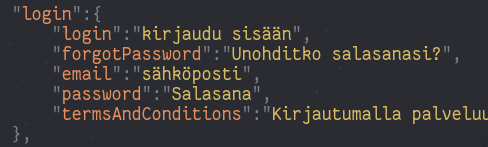
\includegraphics[width= 15cm, height=5cm]{src/public/jsonfixed.png} \\
\medskip
Kuva starttaamon suomenkielisen sisäänkirjautumissivun käännöksestä.
\medskip

Kuvassa näkyy sivun sisäänkirjautumissivun (engl. login) käyttämät suomenkieliset käännökset. Avain on englanniksi kirjoitettu merkkijono, jolla käyttöliittymä hakee käännökset. Arvo on merkkijono mikä ilmenee käyttöliittymälle.
Esimerkiksi saksankielisessä käännöstiedostossa arvo käännettäisi saksaksi.

\medskip

Kielen vaihtoon tarvitaan valikko, josta käyttäjä voi valita millä kielellä hän haluaa käyttää nettisivua. 
Tähän päätin rakentaa laskuvalikon, jossa eri kielet ovat kuvattuna lipuilla.
\medskip





\medskip

\includegraphics[width= 5cm, height=10cm]{src/public/locale_laskuvalikko.png} \\
\medskip
Kuva Laskuvalikosta.
\medskip

Kuvassa näkyy laskuvalikko, jossa kielet on esitetty lippuina.
%Ne ovat kuvattuna lippuina, koska eri kielillä on eri nimet toisille kielille. Mutta 
Liput toimivat nopeina visuaalisina vihjeinä, jotka auttavat käyttäjiä tunnistamaan haluamansa kielen.
Kuvassa olevaan laskuvalikkoon voi lisätä kieliä helposti, mutta usean kielen lisääminen tuo ongelmia käyttöliittymän kanssa, koska laskuvalikko kasvaa ainoastaan alaspäin.
Jos sovellukseen pitäisi lisätä monta eri kieltä, laskuvalikon pitäisi pystyä kasvamaan myös sivusuunnassa ja siihen pitäisi lisätä hakemisto, millä käyttäjä voi hakea haluttua kieltä.
\medskip



\subsection*{Viikon Yhteenveto}


Viikkojen aikana opin käyttämään i18n kirjastoa ja ymmärsin miten käännökset ja lokalisointi toimii nettisivuilla.
Käännökset tämän kokoiseen projektiin on iso työ ja niiden toteuttamiseen kului useita viikkoja.
I18n kirjaston kanssa oli helppo tehdä työtä ja sen dokumentaatio oli kattava.
\medskip

Sovelluksella on nyt keskitetty paikka missä kaikki julkipuolen teksti on, ja koska käännökset on eritelty niille sivuille mihin ne kuuluvat on niiden etsiminen helppoa.
Keskitetty tekstipankki auttaa sovelluksen kehittämisessä tulevaisuudessa, sillä jos haluaa etsiä tekstiä sivuilta ei tarvitse alkaa etsimään komponentteja missä teksti sijaitsee, vaan etsiä se käännöstiedostosta.\medskip

Laskuvalikkoon kielien lisääminen on helppoa, mutta liian monen kielen lisääminen tekee valikosta vaikeakäyttöisen, sillä se kasvaa vain alaspäin.
Laskuvalikkoa voi jatkokehittää lisäämällä siihen ominaisuus, jolla käyttäjä voisi hakea kieliä ja kasvattaa valikkoa sivusuuntaisesti kun tarpeeksi monta kieltä on lisätty.



\newpage




























\tsection{\section}{meteor(Viikko 6)}                          % --------------------------------------------------  VIIKKO 6 -------------------------------------------------- %   
meteorin kanssa tekemistä

\subsection*{meteor}
meteor yleisesti
frontend agnostic framework. voi integroida mihin tahansa frontendiin
open source jos mongodb ei lasketa.
käyttää publisher-subscribe patternia, joka päivittää käyttöliittymän jos tietokantaan tulee muutoksia
\medskip


\subsection*{methodit}
mikä on method ja miski se on olemassa
% meteorin rajapinnat server-client yhteyksissä
\medskip

miten methodeja käytetään projektissa
% kun pitää sanoa serverille että jotain pitää tehdä tai jotain pitää hakea
\medskip


\subsection*{subscriber publisher}
mikä on ja miksi
% meteorin ratkaisu databasejen kanssa tekemiselle
\medskip


miten projekti hyötyää tästä
% aina kun data päivittyy servulla niin tarvittavat komponentit päivittyy automaattisesti
% yksinkertaiset db queryt ei tarvitse erillistä methodia vaan toimii vain publisher subscribe mallilla meteorissa
% vähentää methodien määrää ja kasvattaa koodin luettavuuttaa
\medskip

\subsection*{yhteenveto}
submary mitä tehtiin
\medskip

\newpage

















% https://www.mongodb.com/nosql-explained/nosql-vs-sql#what-are-the-benefits-of-nosql-databases

\tsection{\section}{nosql (Viikko 7-8)}                          % --------------------------------------------------  VIIKKO 7-8 -------------------------------------------------- %   
mitä tehtiin viikolla?

mikä on nosql kanta
toisin kun relatiiviset joilla on teitty row ja collumni määrä non sql voi olla esim. avain-arvo dockumentti graafi jne
sql schma on rigid toisin kun nosql jossa se voi vahdella
\subsection*{mongodb}
mongo projektissa ja miten sen kanssa tehdään juttuja 


\newpage
























\tsection{\section}{uusi ominaisuus (Viikko 10-11)}                          % --------------------------------------------------  VIIKKO 10-11 -------------------------------------------------- %   
progressio multi multi input

\subsection*{selitys featuresta}


\subsection*{toteutus}
react apex charts pystyi lisäämään vaan toisen seriessin


\subsection*{user schema päivitys}
schema päivitys. measurableThing > measurableThings.  
rajapinnat on tyypitetty joten pitää niitä muuttaa että voi toimia.
pitää muuttaa miten käyttöjiä luodaan. ja miten niitä päivitetään
pitää lisätä joku tapa millä lisätä useampia measurableThing eikä vain yhtä
\medskip

user migration. pitää migratoida kaikki aktiiviset asiakkaat measurableThings muotoon.
\medskip





\subsection*{yhteenveto}
miten meni ja miten onnistuin.
\newpage























\tsection{\section}{jotain bullshit (Viikko 12)}                          % --------------------------------------------------  VIIKKO 12 -------------------------------------------------- %   
\iffalse

joku teema pitäis keksia vko 12
raportin luonti?
    tiedostojen tekeminen?

itse viikolla säädettiin ton saman progression kanssa mutta en halua laittaa 3vk samaan hommaaan

feature integration?
raportinteko feature ja progressio featuren merge
en ole maininnut siitä että tein itse sen raportin teon mutta en tidä pitääkö
tämä voisi olla raportin teko aihe ja sitten sen yhdistäminen progressio hommaan?
emt saanko palkoo kirjoitettua sillä se olis 100% casea 

mutta pitttää miettiä


\fi


\newpage

















\tsection{\section}{docker ja siirrettävä kehitysympäristö (Viikko 13)}                          % --------------------------------------------------  VIIKKO 13 -------------------------------------------------- %   
docker compose että saahaan kaikki siistit jutut tehtyy

\subsection*{kontitus}
\subsection*{docker}
\subsection*{docker-compose}
\subsection*{miten tein testiympäristöön}
\subsection*{yhteenveto}

\newpage






\end{document}
